\documentclass[a4paper,12pt]{article}

\usepackage[utf8]{inputenc}

\usepackage[parfill]{parskip}

\usepackage[T1]{fontenc}
\usepackage[french]{babel}
\usepackage{array,multirow,makecell}
\usepackage{longtable}
\usepackage{setspace}
\usepackage{makecell}
\setcellgapes{1pt}
\makegapedcells
\usepackage[table]{xcolor}
\renewcommand*{\emph}[1]{\textcolor{green}{#1}}
\newcolumntype{R}[1]{>{\raggedleft\arraybackslash }b{#1}}
\newcolumntype{L}[1]{>{\raggedright\arraybackslash }b{#1}}
\newcolumntype{C}[1]{>{\centering\arraybackslash }b{#1}}
\usepackage{amsfonts}
\usepackage{fullpage}
\usepackage{graphicx}
\usepackage{float}
\usepackage{geometry}
\usepackage{amsmath}
\usepackage{amssymb}
\usepackage{xspace}
\usepackage{epstopdf}

% -----------------------------------------------------
\begin{document}

    \begin{titlepage}

        \begin{center}

            \title{\Huge INFO-F209 Projets d’informatique 2 \\
            [1 cm] Software Requirements Document \\ 
            L-type\\[2 cm]}
            \author{Aïssa ABDOUL-AZIZ \\[0,2 cm] Kokou ADEGNON \\[0,2 cm] Jeremy BARBER \\[0,2 cm] Helin DEMIREL \\[0,2 cm] Camelia ELKENZE \\[0,2 cm] Alexandre KINSOEN \\[0,2 cm] Salim Latoundji \\[0,2 cm] Mario MASSIMETTI \\[0,2 cm] Martin VANNESTE \\ [2 cm]}
            \date{Décembre 2020}

            %
\includegraphics[width = 40mm]{ulb.png}

        \end{center}

    \end{titlepage}

    \maketitle

\newpage

\tableofcontents

\newpage

% -----------------------------------------------------

\section{Introduction}

L’objectif de ce projet consiste en la réalisation d'un jeu d'action de style shoot 'em up en multijoueur. Dans ce jeu, un ou deux joueurs doivent parcourir plusieurs niveaux en détruisant les ennemis qui se présentent devant eux, tout en esquivant les tirs provoqués par ces derniers. Les vaisseaux dirigés par les joueurs peuvent récupérer des bonus d’armement lâchés par leurs nombreux adversaires pour mieux les éliminer. Le but étant de terminer tous les niveaux sans perdre toute ses vies. En effet, un joueur en possède un nombre déterminé. Si le projectile d'un joueur touche un ennemi, son score est augmenté. Et à la fin d'une partie, le score de chaque utilisateur est mis à jour dans son compte.

En dehors du jeu, un utilisateur a la capacité de gérer sa liste d'amis, de discuter avec d'autres utilisateurs et de consulter le classement général des joueurs.

Le jeu ne sera exécutable que sous le système d'exploitation Linux.

\subsection{Glossaire}
Shoot them up : "abattez-les tous", genre de jeu vidéo

\subsection{Historique}
Historique \emph{de notre travail}

\section{Besoins utilisateur}

\subsection{Besoins fonctionnels}

% ajoute de l'image

\begin{figure}[h!]
\centering
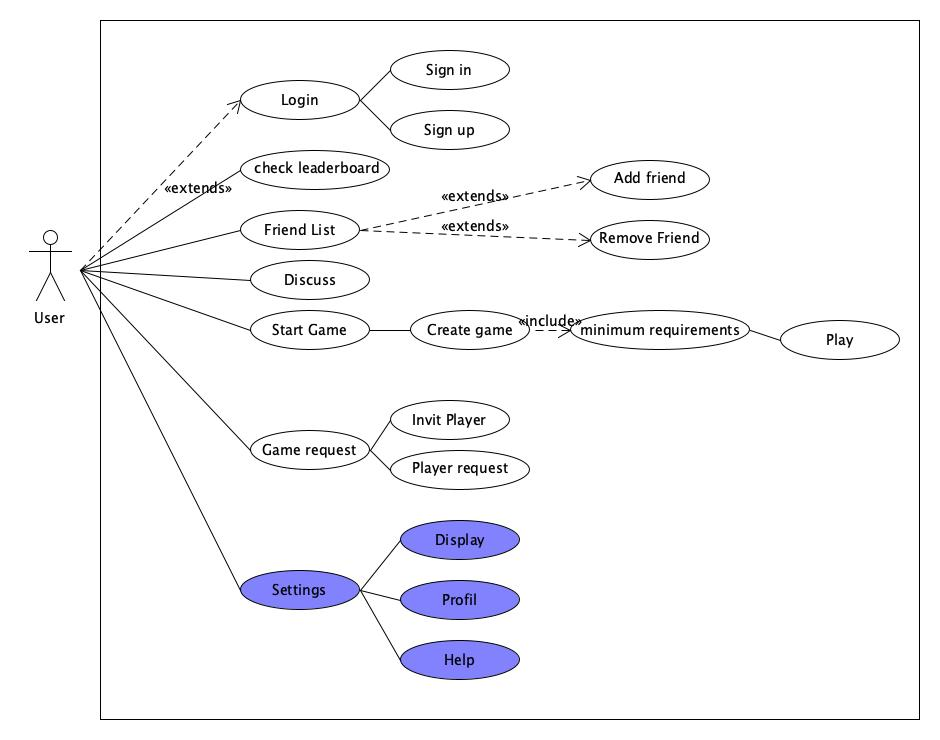
\includegraphics[width=10cm]{UserUseCase1}
\caption{Diagramme de use case coté utilisateur}
\label{fig:UerUseCase}
\end{figure}

\subsubsection{Connexion}
En lançant le programme, l'utilisateur est invité à s'inscrire ou se connecter.

A l'inscription, un pseudonyme unique et un mot de passe lui seront demandé tant que le pseudo entré est déjà pris par quelqu'un d'autre.

Dans le cas de la connexion, on invite l'utilisateur à saisir son pseudo et son mot de passe tant que le pseudo est inexistant ou que le mot de passe ne correspond pas. Après s’être connecté l'utilisateur accède au menu principal.

Dans les deux cas, une option de retour à la page d'accueil sera disponible.

\subsubsection{Menu principal}

- Discuter:

La liste des chats existant est présentée à l'utilisateur, il a le choix de discuter dans un chat existant ou d'en créer un nouveau avec un utilisateur. 

L'utilisateur peut aussi voir si il a de nouveaux messages non-lus.\\

- Consulter amis:

La liste des amis de l'utilisateur est affichée lorsque cette option est sélectionnée. Il peut supprimer un ami, en ajouter un nouveau et aussi voir ses demandes d'amis. 

La suppression d'un ami X par l'utilisateur Y implique la suppression de Y dans la liste d'amis de X. 

L'ajout d'un ami est en fait une invitation. La personne sera l'ami de l'utilisateur seulement si elle accepte sa demande. \\

- Consulter le classement:

Le classement affiche le score de tout les utilisateurs. Si il le souhaite, l'utilisateur peut afficher seulement le classement de score de ses amis. \\

-Envoyer une demande de jeu:

L’utilisateur a la possibilité d’inviter un autre utilisateur, avec un pseudonyme valide, à rejoindre une partie. Si ce dernier est connecté et qu’il n’est pas déjà entrain de jouer, il a possibilité d’accepter ou de refuser la demande. S’il accepte la connexion entre les deux joueurs sera établie, s’il refuse l’hôte ne sera pas averti. \\

-Consulter les demandes de jeu:

Lors d’une consultation de la liste d’invitations, la possibilité est laissée à l’utilisateur d’accepter ou de décliner l’invitation dans le cas ou une invitation est présente dans la liste.Ainsi, accepter une invitation transfère l’utilisateur dans le lobby de l’hôte si ce lobby n’a pas atteint son nombre maximum de joueurs. L’invité ne peut pas modifier les paramètres que le premier joueur aura choisi.A l’inverse refuser une invitation n’avertit pas l’hôte. \\

-Lancer une partie:

Le lancement d’une partie se fait lorsque l’utilisateur crée une partie en gardant les paramètres par défauts ou en les redéfinissants.

- Paramètres:

Dans les paramètres, l'utilisateur peut consulter les règles du jeu avec le bouton "Help". Il peut également configurer ses préférences audio, visuel, ainsi qu'accéder à son profil. Dans son profil, il peut consulter ses informations de compte et s'il le souhaite, changer son mot de passe.

\subsubsection{Création de partie}
La création d'une partie est une option qui envoie l'utilisateur vers une fenêtre de personnalisation permettant de modifier les paramètres du jeu.
Cette fenêtre contient déjà des paramètres par défauts.
S'il le souhaite l'utilisateur peut définir :

-Le nombre de joueur: 

Un joueur a la possibilité de choisir entre un ou deux participants.Dans le cas où le nombre de participants équivaut à deux il aura la possibilité d'entrer un pseudo valide et la partie ne se lancera que si le joueur invité accepte la demande de jeu. \\

-La difficulté de la partie: 

Chaque partie est composée de plusieurs niveaux qui auront chacun plusieurs niveaux de difficultés.  \\

-La probabilité d'apparition des bonus:

L'utilisateur a le choix de gérer la probabilité qu'aura un ennemi de lâcher un bonus après sa destruction. \\

-Le tir allié: 

La possibilité d'activer le tir allié ne peut être accordé que dans le cas où le nombre de joueur est supérieur à un.
Dans ce premier scénario le joueur a le droit de choisir s'il souhaite que les projectiles de l'invité soit inoffensifs ou non. Cette option vaut pour les deux joueurs. \\

-Le nombre de vies: 

Il est laissé à l'utilisateur le choix de posséder jusqu'à cinq vies. \\

Une fois les paramètres validés, si une demande de jeu à un autre joueur a été envoyée le joueur est dirigé vers une salle d'attente en attendant la réponse du second utilisateur. Faute de quoi, le jeu commence directement.

\subsection{Besoins non fonctionnels}

\newpage

\section{Besoins système}
\subsection{Besoins fonctionnels}
\subsubsection{Gestion des comptes}
Les comptes sont stockés dans une base de données. Les différentes demandes d'accès à la base de données sont traitées par le serveur. En effet, celui-ci permet la liaison entre le compte et l'utilisateur.

- Accès:

Lors de la création d'un compte, la disponibilité du pseudo est vérifiée par le serveur. Si celui-ci n'est pas trouvé, un nouveau compte est bien créé et ajouté dans la base de données.

Lors de la connexion, c'est encore le serveur qui vérifie que le pseudo et le mot de passe saisis correspondent à un compte existant.

- Contenu d'un compte:

Chaque compte possède des informations sur l'utilisateur auquel il appartient, notamment ses identifiants(pseudo, mot de passe). Son score est aussi présent pour qu'il apparaisse dans le classement général des joueurs. Il a aussi une liste d'amis qu'il peut consulter à tout moment.

\subsubsection{Création de partie}


\subsubsection{Chat}


\subsubsection{Gestion des amis}

- Ajout: Lorsque l'utilisateur voudra ajouter un ami, le serveur fera des vérifications et enverra la demande, si elle est valide, à la personne concernée. Si la demande est acceptée, la liste d'amis des deux utilisateurs est mise à jour par le serveur.

- Suppression: Le serveur fait une recherche de l'ami à supprimer et efface dans la liste d'amis de celui-ci, l'utilisateur ayant fait la demande de suppression. Ensuite, l'ami est effacé dans la liste de l'utilisateur.


\subsubsection{Classement}

Après chaque partie, le serveur met à jour le score des joueurs si ils ont battu leur record de meilleur score.

\subsection{Besoins non fonctionnels}

\newpage
\section{Annexes}
\subsection{ Description du diagramme use case utilisateur}

\begin{center}
\begin{longtable}{|p{1,5cm}||p{3,5cm}|p{3,5cm}|p{3,5cm}|p{3,5cm}|}
\hline
\rowcolor{green}
USE CASE   &\center{Pré-conditions}   & \hfill Post-conditions \hfill\null & Cas Général & Cas exceptionnels\\
\hline
\hline
\textbf{Sign in}      & L'utilisateur doit être enregistré dans la base de données  & L'utilisateur est connecté à sa base de données et le menu principal est affiché & L'utilisateur déjà enregistré se connecte à son compte en tapant son nom d’utilisateur et mot de passe. Le système vérifie que les données soient correctes et donne accès au compte du client.  & Si l’identifiant ou le mot de passe sont incorrectes, le système affiche un message d'erreur a l'utilisateur. \\
\hline
\hline
\textbf{Sign up}     & L'utilisateur n'est pas présent dans la base de données   & Ajout d'un compte dans la base de données et affichage du menu principal & L'utilisateur crée un compte en introduisant un pseudo et un mdp  & Si les données entrées ne respectent pas le format requis ou que le nom d'utilisateur est déjà utilisé, un message d'erreur est affiché et l'utilisateur doit recommencer l'action jusqu'à ce que ce soit valide \\

\hline
\hline
\textbf{Create game}    & L'utilisateur doit être enregistré dans la base de données  & Possibilité de sauvegarder les options requises  & L'utilisateur peut lancer une partie après avoir rempli les conditions minimales  & Néant \\
\hline
\hline
\textbf{Invite player} & L'utilisateur doit être enregistré dans la base de données   & Etablissement de la connexion via le serveur entre l’hôte et l’invité. & Inviter un joueur avec son pseudo & Invitation via pseudo qui n’existe pas. \\
\hline
\hline
\textbf{Player request}  & Recevoir une invitation via le serveur.
L'utilisateur doit être enregistré dans la base de données   & Etablissement de la connexion via le serveur entre l’hôte et l’invité.  & Accepter/ Refuser une invitation de partie  & La connexion échouera si :
Accepter une invitation dont l'hôte n’est plus connecté.
Rejoindre un salon complet. \\
\hline
\hline
\textbf{Check Leaderboard}  & L'utilisateur doit être enregistré dans la base de données   & \hfill Néant  \hfill\null &Le joueur peut consulter le classement des meilleurs scores en envoyant une requête au serveur qui va lui renvoyer les informations  & Néant \\
\hline
\hline
\textbf{View friend list }   & L'utilisateur doit être enregistré dans la base de données   & Néant  & Consultation de liste d'ami dans la base de données. & Néant \\
\hline
\hline
\textbf{Chat}     & L'utilisateur doit être enregistré dans la base de données   & Le serveur effectue les liaisons entre les utilisateurs  & Envoyer et recevoir des messages avec n'importe quel pseudo.  & Néant \\
\hline
\hline
\textbf{Add friend}    & L'utilisateur doit être enregistré dans la base de données   & Si invitation acceptée, ajout d'amis dans la base de donnée (bidirectionnel).  & Entrer le pseudo d’un ami. Le système va rechercher dans la base de données si le pseudo existe et l’ajouter.  & Ajouter un ami qui n’existe pas (affiche une erreur).\\
\hline
\hline
\textbf{Delete friend}    & L'utilisateur doit être enregistré dans la base de données et avoir au moins un ami.   & Suppression d’amis(de la liste d’amis) de la base de données.  & Entrer le pseudo d’un ami. Le système va rechercher dans la base de données si le pseudo existe et le supprimer.  & Supprimer un ami qui n’existe pas (affiche une erreur). \\
\hline
\hline
\textbf{Settings}     & L'utilisateur doit être enregistré dans la base de données   & Mise à jour des changements  & L'utilisateur modifie des parametres de son profil de l'affichage ou du son  & Néant\\
\hline
\hline
\textbf{Ship’s controls}  & Charger une partie/créer une partie.   & Actualisation de l’état de jeu.  & Bouger, tirer recevoir des bonus.  & Néant\\
\hline
\hline
\textbf{Leave party}      & Être en train de jouer   & Retour au menu principal  & Le joueur arrête la partie en cours.  & Néant\\
\hline
\hline
\textbf{Help}      & Etre connecté   & Néant  & Les règles principales du jeu sont affichées au joueur & Néant\\
\hline
\hline
\textbf{Leave game}      & Etre connecté   & Fermeture du jeu  & L'utilisateur est connecté et veut quitter le jeu  & L'utilisateur est connecté et force sa sortie du jeu (CTRL+C, ...)\\
\hline
\end{longtable}
\end{center}


\end{document}
